\chapter{Risolutori basati sul modello MIP}
La seconda via studiata per risolvere in maniera esatta il TSP è la formulazione del problema come problema di programmazione lineare mista intera, in cui alcune variabili sono vincolate all'interezza, mentre su altre tale vincolo è rilassato e possono assumere valori continui. Il modello viene poi risolto con il solver commerciale CPLEX, disponibile gratuitamente per uso accademico e di studio. Esistono vari MIP solver commerciali e open source, che si basano sostanzialmente su un branch-and-cut eseguito sul rilassamento continuo del problema, in cui ad ogni nodo un pool di tagli ed euristici viene applicato sulla soluzione valutata.

\section{Modello MIP del TSP}\label{sec:relaxelsecs}
Il modello MIP del TSP è riportato nell'introduzione della presente relazione. Il modello proposto è computazionalmente intrattabile; la causa principale di questa situazione risiede nel numero dei vincoli di aciclicità. Possiamo quindi rilassare il problema eliminando i SECs, e risolvere il problema così modificato. In genere, una soluzione al problema rilassato conterrà dei sottocicli; in tal caso possiamo individuarli, vietarli mediante appositi vincoli aggiunti come cutting planes e risolvere il nuovo problema. L'idea alla base di tale procedimento è che solo una piccola parte dei SECs sono effettivamente necessari per la corretta risoluzione del modello, mentre la maggior parte di loro non verrà mai violata da soluzioni di sufficiente qualità, pertanto la loro inclusione risulterebbe solo in un appesantimento del modello MIP.

\subsection{Preprocessing}
Il subgradiente lagrangiano fornisce un lower bound rispetto alla soluzione ottima, mentre varie tecniche euristiche (cap. \ref{sec:capheur}) permettono di calcolare una soluzione ammissibile, quindi un upper bound al valore dell'ottimo. Possiamo sfruttare queste informazioni per ``aiutare'' la risoluzione del modello, imponendo al risolutore di escludere dal calcolo le variabili corrispondenti agli archi che possiamo determinare a priori non saranno presenti nella soluzione ottima. Questo procedimento si può effettuare nella maniera descritta in sezione \ref{sec:riduzionelati}.

Un altro intervento preliminare che possiamo compiere è fornire al solver una soluzione intera ammissibile da cui partire per un ``raffinamento'' verso la soluzione ottima. Anche in questo caso, la soluzione iniziale si può calcolare con un algoritmo euristico.

\section{Risoluzione iterativa}
Il primo procedimento di risoluzione analizzato consiste nell'applicare in maniera diretta la procedura descritta nella sezione \ref{sec:relaxelsecs}. L'algoritmo itera i seguenti passi:
\begin{enumerate}[noitemsep]
  \item risoluzione del modello rilassato per eliminazione dei vincoli SEC;\label{iterpasso1}
  \item ricerca di sottocicli nella soluzione ottenuta;
  \begin{enumerate}[noitemsep]
    \item se presenti, aggiunta dei relativi vincoli al modello e ritorno al passo \ref{iterpasso1};
    \item altrimenti, è stato individuato il ciclo hamiltoniano di costo minimo, e l'algoritmo termina.
  \end{enumerate}
\end{enumerate}

Questa procedura implementa un metodo duale, che nel cammino verso l'ottimo globale individua soluzioni di costo migliore dell'ottimo, ma non ammissibili in quanto contenenti sottocicli. La prima soluzione composta di un solo ciclo sarà quindi la soluzione ottima. Tale procedimento comporta che, ad ogni iterazione, al passo \ref{iterpasso1} venga risolto da zero un modello corrispondente al modello dell'iterazione precedente, con l'aggiunta dei vincoli di eliminazione di sottociclo violati dalla soluzione ottima dell'iterazione precedente. Di conseguenza, iterazione dopo iterazione il modello sarà sempre più computazionalmente pesante.

Per velocizzare le operazioni, i solver forniscono funzionalità di \textit{presolving}, che, prima del nodo radice del branch-and-cut interno, analizzano il modello e tentano di semplificarlo, identificando e rimuovendo variabili e vincoli ridondanti o inefficaci.

La ricerca di sottocicli viene effettuata individuando le componenti connesse nella soluzione, e inserendo un vincolo \ref{eqn:secs} nel modello per ciascuna di esse.

\section{Risoluzione con callback ``alla Miliotis''}
Un secondo metodo di risoluzione, la cui implementazione in CPLEX è resa possibile dal meccanismo delle callback, è quello proposto da Miliotis \citep{miliotis1978using}, che valuta l'incumbent nel corso della risoluzione, invece che al termine della procedura come fa il metodo precedente. In particolare, non appena ad un nodo viene individuata una soluzione intera, su di essa viene immediatamente valutata la presenza o meno di sottocicli, in maniera identica a quanto fatto con il metodo iterativo. Se presenti, essi vengono aggiunti come tagli, altrimenti l'esecuzione può terminare, avendo trovato l'ottimo globale. Tale procedura segue un metodo primale, ovvero che attraversa una serie di soluzioni ammissibili subottime fino a raggiungere la soluzione ottima.

Il meccanismo delle callback è un paradigma di implementazione che prevede l'esecuzione di un metodo fornito dallo sviluppatore al verificarsi di un particolare evento, per gestire la situazione nella maniera più appropriata. Nel nostro caso, CPLEX fornisce callbacks per eventi diversi che possono occorrere durante la risoluzione di un modello, o per accedere ad alcune informazioni sullo stato della risoluzione (\textit{informative callbacks}). Per motivi di segretezza commerciale alcune funzionalità proprietarie di CPLEX vengono tuttavia disabilitate con l'uso delle callback. Le callback che permettono di analizzare l'incumbent sono dette in CPLEX \textit{lazy constraints}, perché invocate solo quando è presente una soluzione, al contrario delle callback di tipo \textit{user cut} che vengono valutate ad ogni nodo dell'albero di branching.

\section{Risoluzione con callback sulla soluzione frazionaria}
Abbiamo menzionato la possibilità di invocare delle callback ad ogni nodo dell'albero decisionale sulla soluzione frazionaria corrente, valutando l'eventuale violazione dei vincoli di eliminazione dei sottocicli con le callback \textit{user cut}.

In generale, una soluzione frazionaria avrà conterrà nodi su cui incidono un numero di archi maggiore di 2, ma pesati in maniera tale da rispettare comunque il vincolo di grado. Il problema da risolvere in una soluzione così composta è un problema di flusso massimo su archi di capacità 1 (essendo le variabili degli archi binarie), in cui è necessario imporre che per ogni insieme di nodi $S$ vi siano almeno due archi che collegano $S$ all'insieme complementare $V \setminus S$. L'implementazione di tale procedimento è stata invece effettuata basandoci sul problema duale del max-flow, ovvero la determinazione del taglio minimo nel grafo, usando le funzioni per il calcolo del min cut implementate nel software Concorde. Tali metodi richiedono la connessione del grafo. Se tale condizione è verificata, il metodo \texttt{CCmincut} ritorna l'insieme di nodi $S$ costituenti un taglio minimo nel grafo così partizionato in $S$ e $V\setminus S$; in questo caso, si impone il vincolo
\begin{equation}
  \sum_{e \in \delta(S)}x_e \geq 2, \label{eqn:flowconst}
\end{equation}
per rendere connesso il sottografo $S$ con il resto dei nodi. Se invece il grafo con archi frazionari non è connesso, si aggiungono vincoli mirati a spezzare le componenti connesse e rendere il grafo connesso.

Poiché le user cut callbacks vengono invocate ad ogni nodo dell'albero decisionale, esse possono rallentare enormemente l'esecuzione, rendendo impraticabile la risoluzione di problemi di medio-grandi dimensioni. Una possibile strategia è quella di applicare la ricerca dei vincoli violati solo nei nodi a bassa profondità, o su una frazione dei nodi scelta con qualche criterio (ad es: in una certa percentuale di nodi, scelti a caso).

\section{Risultati computazionali}
\afterpage{%
    \clearpage% Flush earlier floats (otherwise order might not be correct)
    \thispagestyle{empty}% empty page style (?)
\begin{scriptsize}
\begin{landscape}
    \begin{longtabu} to \linewidth {c|rr|rS[table-format=6.2]|rS[table-format=6.2]|rS[table-format=6.2]}
    \toprule
    \multicolumn{3}{c}{} & \multicolumn{2}{c}{Iterativo} & \multicolumn{2}{c}{Lazy constraints cbs.} & \multicolumn{2}{c}{User cut cbs.} \\
%    \cmidrule(r){4-5} \cmidrule(r){6-7} \cmidrule(r){8-9}
    Istanza & UB & LB & $z^*$ & T [s] & $z^*$ & T [s] & $z^*$ & T [s] \\
    \midrule
    \endhead
\label{tab:cplexres}
%\caption{Risultati ottenuti usando CPLEX.}
a280 & 2627 & 2566 & 2579 & 30.28 & 2579 & 2.82 & 2579 & 2.14  \\
ali535 & 208383 & 201237 & 201467 & 5783.06 & 202368 & 3927.78 & & \\
att48 & 10628 & 10603 & 10628 & 0.06  & 10628 & 0.03  & 10628 & 0.03 \\
att532 & 28743 & 27420 & 27684 & 3662.56  & 27706 & 3190.86  \\
berlin52 & 7542 & 7542 & 7542 & 0.00 & 7542 & 0.01 & 7542 & 0.00 \\
bier127 & 119003 & 117431 & 118282 & 1.89 & 118282 & 0.44  & 118282 & 0.63  \\
ch130 & 6178 & 6076 & 6110 & 0.91 & 6110 & 0.27  & 6110 & 0.45  \\
ch150 & 6548 & 6491 & 6528 & 3.85 & 6528 & 0.90 & 6528 & 1.13  \\
d198 & 15863 & 15712 & 15780 & 136.32 & 15780 & 6.19  & 15780 & 2.82 \\
d493 & 35987 & 34829 & 34957 & 3609.99 & 35004 & 3872.03 &  &  \\
d657 & 50330 & 48456 & 48887 & 4117.63 &  & 3600.75 &  & \\
eil101 & 634 & 628 & 629 & 0.31 & 629 & 0.11  & 629 & 0.20 \\
eil51 & 427 & 423 & 426 & 0.12 & 426 & 0.03  & 426 & 0.03  \\
eil76 & 543 & 537 & 538 & 0.05 & 538 & 0.02  & 538 & 0.01  \\
fl417 & 11961 & 11790 & 11861 & 1644.89 & 11869 & 3657.51 &  & \\
fri26 & 937 & 937 & 937 & 0.01 & 937 & 0.00  & 937 & 0.00  \\
gil262 & 2438 & 2355 & 2378 & 88.63  & 2378 & 118.71  & 2378 & 90.31 \\
gr137 & 70496 & 69121 & 69853 & 5.12 & 69853 & 0.60 & 69853 & 0.31  \\
gr17 & 2085 & 2085 & 2085 & 0.01 & 2085 & 0.00 & 2805 & 0.00  \\
gr202 & 41069 & 40055 & 40160 & 21.58  & 40160 & 2.22 & 40160 & 1.78  \\
gr21 & 2707 & 2707 & 2707 & 0.00 & 2707 & 0.00 & 2707 & 0.00 \\
gr229 & 137652 & 133318 & 134602 & 175.39  & 134602 & 57.85 & 134602 & 32.97 \\
gr24 & 1272 & 1272 & 1272 & 0.01 & 1272 & 0.01 & 1272 & 0.00 \\
gr48 & 5046 & 4959 & 5046 & 0.47  & 5046 & 0.09 & 5046 & 0.10 \\
gr666 & 304907 & 292494 & 294358 & 3444.76 & 294358 & 3852.26 &  & \\
gr96 & 55589 & 54571 & 55210 & 2.27 & 55210 & 0.33 & 55210 & 0.28 \\
hk48 & 11461 & 11442 & 11461 & 0.01 & 11461 & 0.01 & 11461 & 0.00  \\
kroA100 & 21282 & 20937 & 21282 & 1.44 & 21282 & 0.27 & 21282 & 0.22 \\
kroA150 & 26815 & 26299 & 26524 & 16.33  & 26524 & 3.05 & 26524 & 3.57 \\
kroA200 & 29575 & 29065 & 29368 & 75.04 & 29368 & 105.74 & 29368 & 133.07 \\
kroB100 & 22278 & 21834 & 22141 & 3.28  & 22141 & 0.52 & 22141 & 0.57 \\
kroB150 & 26445 & 25733 & 26130 & 74.43 & 26130 & 41.63 & 26130 & 45.22 \\
kroB200 & 30035 & 29165 & 29437 & 33.57  & 29437 & 12.90 & 29437 & 3.89  \\
kroC100 & 20769 & 20473 & 20749 & 1.08  & 20749 & 0.27 & 20749 & 0.27  \\
kroD100 & 21404 & 21142 & 21294 & 0.98  & 21294 & 0.20 & 21294 & 0.30  \\
kroE100 & 22100 & 21800 & 22068 & 2.43  & 22068 & 0.73 & 22068 & 0.62  \\
lin105 & 14379 & 14371 & 14379 & 0.42  & 14379 & 0.25  & 14379 & 0.40 \\
lin318 & 43200 & 41889 & 42029 & 213.63  & 42029 & 31.10 & 42029 & 84.01 \\
p654 & 34905 & 33567 &  &   &  & 1261.05 &  & \\
pcb442 & 53051 & 50500 & 50778 & 1145.56  & 50778 & 44.30 & 50778 & 37.54 \\
pr107 & 44676 & 43681 & 44303 & 0.13  & 44303 & 0.02 & 44303 & 0.02 \\
pr124 & 59087 & 58068 & 59030 & 16.63  & 59030 & 15.36 & 59030 & 0.50 \\
pr136 & 97644 & 95935 & 96772 & 4.65  & 96772 & 0.31 & 96772 & 0.50  \\
pr144 & 58571 & 58158 & 58537 & 11.86  & 58537 & 2.66 & 58537 & 0.89 \\
pr152 & 74021 & 73209 & 73682 & 1.70  & 73682 & 1.91 & 73682 & 0.94 \\
pr226 & 80590 & 80092 & 80369 & 2062.50  & 80369 & 78.51 & 80369 & 3.07 \\
pr264 & 49636 & 49010 &  &   & 49135 & 65.05 & 49135 & 1.06 \\
pr299 & 48816 & 47380 & 48191 & 628.81 & 48191 & 4013.15 & 48231 &  \\
pr439 & 108425 & 105929 & 106978 & 3683.16 & 107250 & 2011.72 &  & \\
pr76 & 108274 & 105120 & 108159 & 12.21 & 108159 & 12.32 & 108159 & 15.35 \\
rat195 & 2371 & 2300 & 2323 & 114.32 & 2323 & 26.84 & 2323 & 9.10  \\
rat575 & 7105 & 6724 & 6773 & 3224.39  & 6773 & 3021.12 &  & \\
rat783 & 9186 & 8773 & 8806 & 3333.15 & 8806 & &   &   \\
rat99 & 1213 & 1206 & 1211 & 0.54 & 1211 & 0.06 & 1211 & 0.06 \\
rd100 & 7913 & 7900 & 7910 & 0.46  &  7910 & 0.35 & 7910 & 0.18  \\
rd400 & 15666 & 15157 & 15281 & 841.03 & 15282 &  & 15302 &   \\
st70 & 675 & 671 & 675 & 0.09  & 675 & 0.06 & 675 & 0.07 \\
swiss42 & 1273 & 1272 & 1273 & 0.01  & 1273 & 0.00  & 1273 & 0.00\\
ts225 & 126809 & 115605 &  &  &  & &  & \\
tsp225 & 4047 & 3879 & 3916 & 165.70  & 3916 & 36.96 & 3916 & 35.26 \\
u159 & 42624 & 41925 & 42080 & 2.16  & 42080 & 1.15 & 42080 & 0.41  \\
u574 & 38334 & 36714 & 36905 & 1230.89 & 36907 & 3741.80 &  & \\
u724 & 43860 & 41653 & 41821 & 3687.35  & 42003 & 3762.89 &  & \\
ulysses16 & 6859 & 6859 & 6859 & 0.00 & 6859 & 0.01  & 6859 & 0.01 \\
ulysses22 & 7013 & 7013 & 7013 & 0.02 & 7013 & 0.00  & 7013 & 0.00 \\
\bottomrule
    \end{longtabu}
%    \end{landscape}
\captionof{table}{Risultati della risoluzione con CPLEX iterativo, con lazy constraint callbacks e user cut callbacks.}% Add 'table' caption
    \end{landscape}
    \clearpage% Flush page
\end{scriptsize}
}
I test riportati sono stati effettuati su una macchina con processore Intel Core i7 quad-core con hyperthreading a 2,40GHz e 4 GB di RAM. Nelle tabella \ref{tab:cplexres} mostriamo i risultati ottenuti con i metodi esatti basati su CPLEX, imponendo un tempo limite di un'ora per ogni soluzione. I valori mancanti indicano che non è stata individuata alcuna soluzione ammissibile nei tempi dati, o che l'esecuzione è stata abortita anticipatamente (soprattutto per eccessivo uso di memoria, nel caso delle user cut callback). I tempi talvolta eccedono i 3600 secondi, a causa dell'implementazione interna a CPLEX del controllo sul time limit. Le user cut callbacks vengono individuate sul 5\% dei nodi dell'albero di branching scelti in maniera casuale.

Si può facilmente notare come nella maggior parte dei casi le soluzioni con callback siano decisamente più performanti rispetto alla soluzione iterativa, con alcune significative eccezioni. Vi sono istanze di taglia elevata che non sono state risolte nei tempi dati; in un caso non è stato nemmeno possibile trovare una soluzione ammissibile, sintomo di come sia consigliabile fornire una soluzione di partenza al solver. In altri casi l'implementazione basata su callbacks ha raggiunto la soluzione ottima, non riuscendo a certificarla nei tempi dati, situazione che con la versione iterativa non si può verificare.

La risoluzione con callback user cut sulla soluzione frazionaria delle istanze più grandi è stata abortita quando l'occupazione di memoria diventava eccessiva.

Mostriamo inoltre due immagini a titolo di esempio su come procede l'aggiornamento dell'incumbent nella versione iterativa (figura \ref{fig:updatingincumbentiter}) e con le callback (figura \ref{fig:updatingincumbent}).

Nella versione iterativa il costo della soluzione incumbent è sempre un lower bound della soluzione ottima, procedendo attraverso soluzioni di costo minore dell'ottimo ma inammissibili, fino a raggiungere la miglior soluzione ammissibile, che sarà la soluzione ottima; nel metodo che fa uso di callback, invece, la risoluzione attraversa soluzioni ammissibili ma subottime, fino a giungere alla soluzione ottima, che dovrà essere certificata.

Vediamo chiaramente come in entrambe le versioni il solver all'inizio aggiorni la migliore soluzione molto velocemente, per poi rallentare vistosamente quando si avvicina all'ottimo globale, fatto poco sorprendente essendo una manifestazione dello stato di problema NP-completo del TSP. Il MIP solver deve infatti attraversare, al caso peggiore, l'intero albero di branching.

\begin{figure}
  \begin{center}
    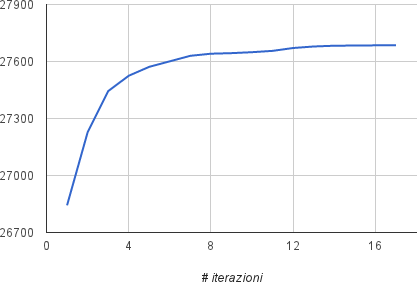
\includegraphics[width=0.48\textwidth]{images/att532iteragg}
    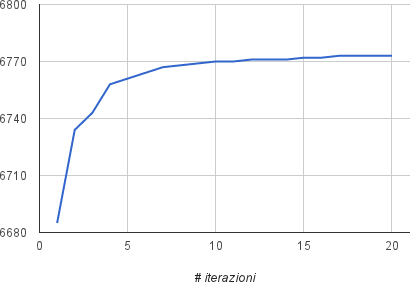
\includegraphics[width=0.48\textwidth]{images/rat575iteragg}
    \caption{Aggiornamento dell'incumbent di \texttt{att532} e \texttt{rat575} nella risoluzione iterativa.}
    \label{fig:updatingincumbentiter}

    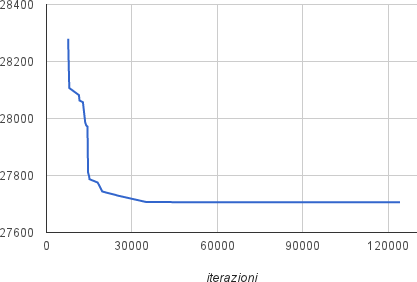
\includegraphics[width=0.48\textwidth]{images/att532aggiornamento}
    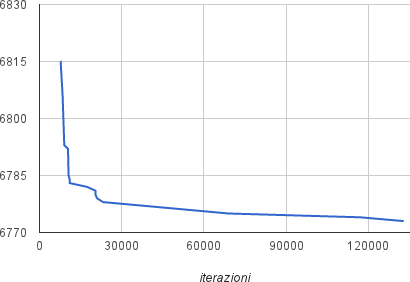
\includegraphics[width=0.48\textwidth]{images/rat575aggiornamento}
    \caption{Aggiornamento dell'incumbent di \texttt{att532} e \texttt{rat575} nella risoluzione con callback.}
    \label{fig:updatingincumbent}
  \end{center}
\end{figure}

In entrambi i casi osserviamo un drastico miglioramento nelle prime iterazioni, che in seguito rallenta vistosamente. Per quanto riguarda \texttt{att532} l'ottimo viene trovato (all'incirca) all'iterazione 56000, mentre l'esecuzione termina con la certificazione dopo oltre 120000 iterazioni. L'ottimo di \texttt{rat575} invece viene trovato all'ultima iterazione prima che CPLEX venga terminato per aver ecceduto il time limit, senza quindi poter essere certificato; anche in questo caso, comunque, il trend dell'aggiornamento ricalca quello di \texttt{att532}, così come, in genere, di tutte le altre istanze. 

\section{Commenti}
La risoluzione con solver MIP permette di attaccare problemi che altrimenti non sarebbero risolvibili con un branch-and-bound classico. La risoluzione con metodo iterativo scandisce lo spazio analizzando le soluzioni in ordine crescente di costo, di modo che la prima soluzione intera senza sottocicli è la soluzione ottima. Soluzioni intere incontrate nella risoluzione precedentemente all'ottimo includono sottocicli, e vanno perciò vietate mediante cutting planes. La risoluzione mediante callback invece procede in maniera primale, individuando soluzioni ammissibili di costo sempre minore, fino a raggiungere la soluzione ottima.  Questo fornisce alla risoluzione con callback un comportamento \textit{anytime}, avendo sempre una soluzione incumbent sin dalla prima soluzione feasible trovata. Nel tempo limite di un'ora assegnato ad ogni istanza, non è sempre stato possibile individuare la soluzione ottima; tuttavia, il metodo con le callbacks ha permesso di individuare soluzioni di costo di poco superiore all'ottimo, fatto non possibile con il metodo iterativo. Come abbiamo visto dai grafici in figura \ref{fig:updatingincumbent}, questo non è comunque una garanzia dell'essere nei pressi della soluzione ottima, ovvero non è possibile stimare il tempo o il numero di iterazioni rimanenti prima di individuare il tour ottimo.

Dal punto di vista delle prestazioni, la risoluzione con callback è più veloce, al costo di una maggiore occupazione di memoria. In particolare, l'uso delle callback sulla soluzione frazionaria aumenta di molto l'occupazione di RAM, essendo invocate ad ogni nodo dell'albero di branching.

Come risolutore di default, in base ai risultati ottenuti con i test precedentemente riportati, la soluzione consigliabile è quella basata sulle callback di tipo \textit{lazy constraints}, essendo quella che rende il miglior compromesso tra prestazioni e requisiti computazionali.

Segnaliamo che in certi casi il solver ha terminato l'esecuzione ad un tempo superiore al tempo massimo assegnato: questo è dovuto al fatto che il controllo sul time limit viene effettuato quando il solver è in uno stato consistente, cosa che talvolta lo porta a ``sforare'' significativamente i limiti assegnati. Altra caratteristica dei solver MIP, dovuta alla loro natura di branch-and-cut, è il loro comportamento erratico che rende impredicibile l'esecuzione; le scelte di branching effettuate all'interno del solver dipendono da molti fattori, spesso al di fuori della possibilità di intervento dell'utente. Oltre a questo, soluzioni come Dynamic Search per l'attraversamento dell'albero sono tenute nascoste all'utente, cosa che limita ulteriormente la possibilità di comprensione dell'esecuzione \footnote{Ad esempio, all'interno di una callback non è possibile ottenere un timestamp, perciò non si può valutare il tempo trascorso ed eventualmente abortire l'esecuzione. Anche il nodo in cui l'incumbent viene aggiornato è tenuto nascosto, e viene mostrato solo il suo valore arrotondato.}.
